\newcommand{\VloadPeak}{\qty{7.67}{\volt}}
\newcommand{\RL}{\qty{1.1}{\kilo\ohm}}
\newcommand{\TL}{\qty{10}{\milli\second}}
\newcommand{\fL}{\qty{100}{\hertz}}

\newcommand{\VZ}{\qty{4.7}{\volt}}
\newcommand{\VoDC}{\qty{2.83}{\volt}}
\newcommand{\IZ}{\qty{3.1}{\milli\ampere}}

\subsection*{5. LTspice Simulation}
All plots and variables are derived from the example circuit provided in the related subsection, which are configured using the component values specified in the laboratory manual.\par
\textit{Note: Related questions are answered at the end of each subsection.}

\subsection*{5.1 Used SPICE Models}
\texttt{.model 1N750 D(Is=.88f Rs=.25 Cjo=175p M=.55 nbv=1.7 bv=4.7 Vj=.75 Isr=1.86n Nr=2\\
Ibv=20.245m Ibvl=1.96m Nbvl=15 Tbv1=-21.3u Vpk=4.7 mfg=OnSemi type=Zener)}\par
\texttt{.model 1N4007 D(Is=90p Rs=40m Cjo=30p N=1.4 TT=5u Iave=1 Vpk=1000 mfg=Diodes\_Inc.\\
type=silicon)}

\subsection*{5.2 Full-Wave Bridge Rectifier}
The purpose of a full-wave bridge rectifier circuit is to convert an AC voltage to a DC voltage. 
As the bridge rectifier rectifies both half-cycles of the input signal into a single polarity, the frequency of the output voltage is doubled relative to the input frequency.
Since two diodes conduct in series during each half-cycle, the circuit has a voltage drop equal to the sum of the forward voltage drops of the two conducting diodes.
To prevent severe voltage sag, a filter capacitance is needed. An example circuit is given in \autoref{fig:circuit-1}.

\begin{figure}[H]
    \centering
    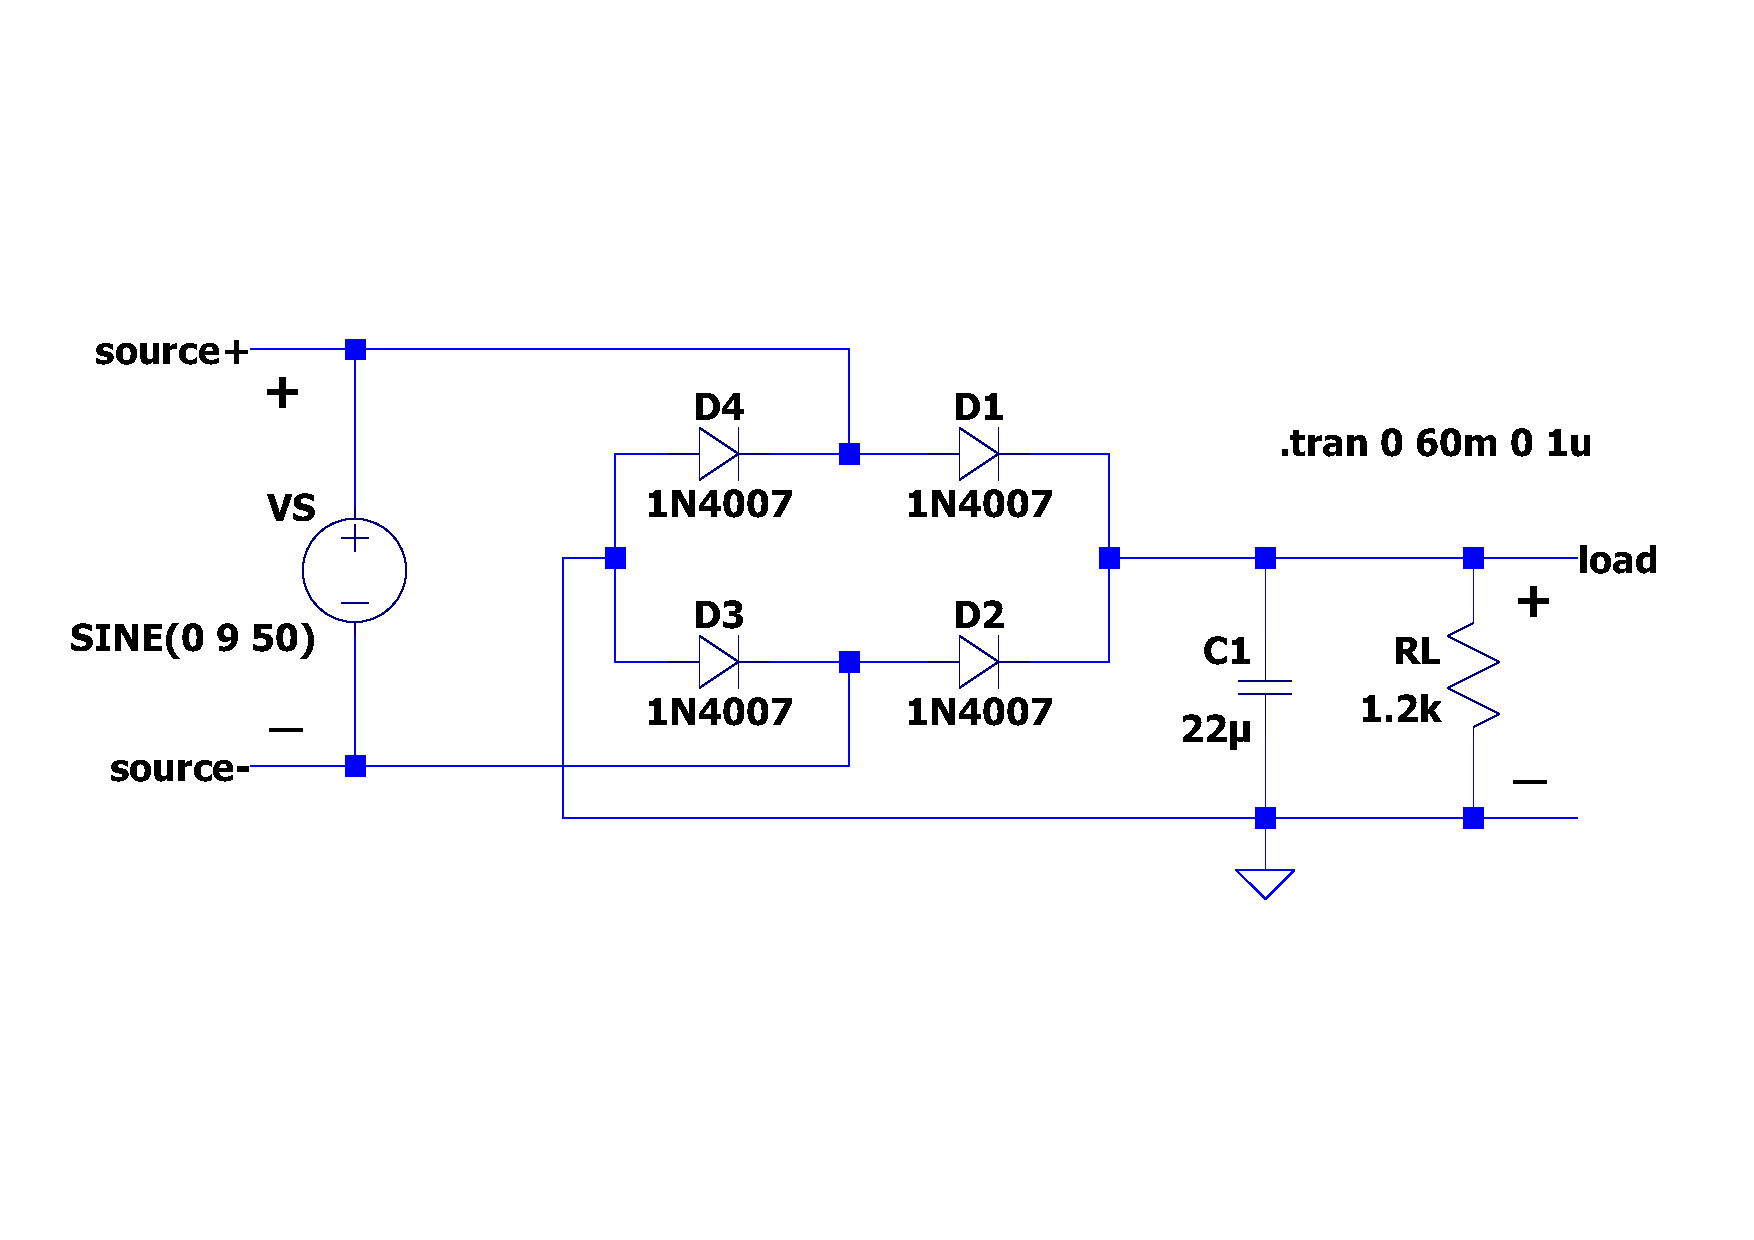
\includegraphics[width=0.7\textwidth]{./figures/circuit-1.pdf}
    \caption{Schematic of full-wave bridge rectifier circuit}
    \label{fig:circuit-1}
\end{figure}

\begin{figure}[H]
    \centering
    \begin{overpic}[width=0.8\textwidth]{./figures/plot-1.pdf}
        \put(58.4,59.5){\scriptsize{$\downarrow$ $V_{L,\text{peak}}$ (\VloadPeak)}}
        \put(55.8,52.7){\footnotesize{$\xleftrightarrow[\quad f_L = \fL\quad ]{T_L = \TL}$}}
    \end{overpic}
    \caption{Input and output voltage waveforms of the full-wave bridge rectifier circuit}
    \label{fig:plot-1}
\end{figure}

\subsubsection*{5.2.1 Questions}
\textbf{a.) } \textit{Determine the peak value and frequency of $v_L$, and compare the results with your calculations in Question-1}\par
\vspace{0.2cm}
\begin{center}
    \begin{tabular}{|c|c|c|c|}
        \hline
        $V_{L,\mathrm{peak}}$ & $f_L$ & \textbf{Number of conducting diodes} \\ \hline
        \VloadPeak & \fL & 2 \\ \hline
    \end{tabular}
\end{center}
\vspace{0.2cm}
-- Output Ripple Frequency ($f_L$): It is the same for both theoretical calculations and simulation results since both rely on the same frequency-doubling formula ($f_L = 2 \times f_s$).\par
-- Peak Load Voltage ($V_{L,\mathrm{peak}}$): The diode forward voltage drop is greater in the simulation because the model accounts for dynamic and non-linear parameters, whereas the theoretical calculation assumes a constant forward voltage drop.
This results in a slightly lower peak load voltage in the simulation compared to hand calculations.\par

\vspace{0.5cm}
\textbf{b.) } \textit{Include the plot showing $v_S$ and $v_L$ in your prelab report.}\par
-- The input and load voltage of the example circuit is given in \autoref{fig:plot-1}.

\subsection*{5.3 Zener Diode Regulator}
In full-wave bridge rectifier circuits, a key limitation is that the peak output voltage ($V_{L,\mathrm{peak}}$) and the peak-to-peak ripple voltage ($V_{rpl,PP}$) are affected by load conditions. 
As the load current increases, the voltage drops across the bridge diodes and series components increase, causing the output voltage to sag. 
To address this limitation and clamp the peak output voltage to a desired, more stable level, a Zener diode regulator can be implemented. 
However, since the excess voltage is entirely dropped across the series resistor ($R_S$), this circuit suffers from poor thermal and power efficiency, especially in high-current applications. 
Despite this inefficiency, it remains a low-cost practical solution for low-current voltage references and basic low-power circuits. An example circuit is given in \autoref{fig:circuit-2}.

\begin{figure}[H]
    \centering
    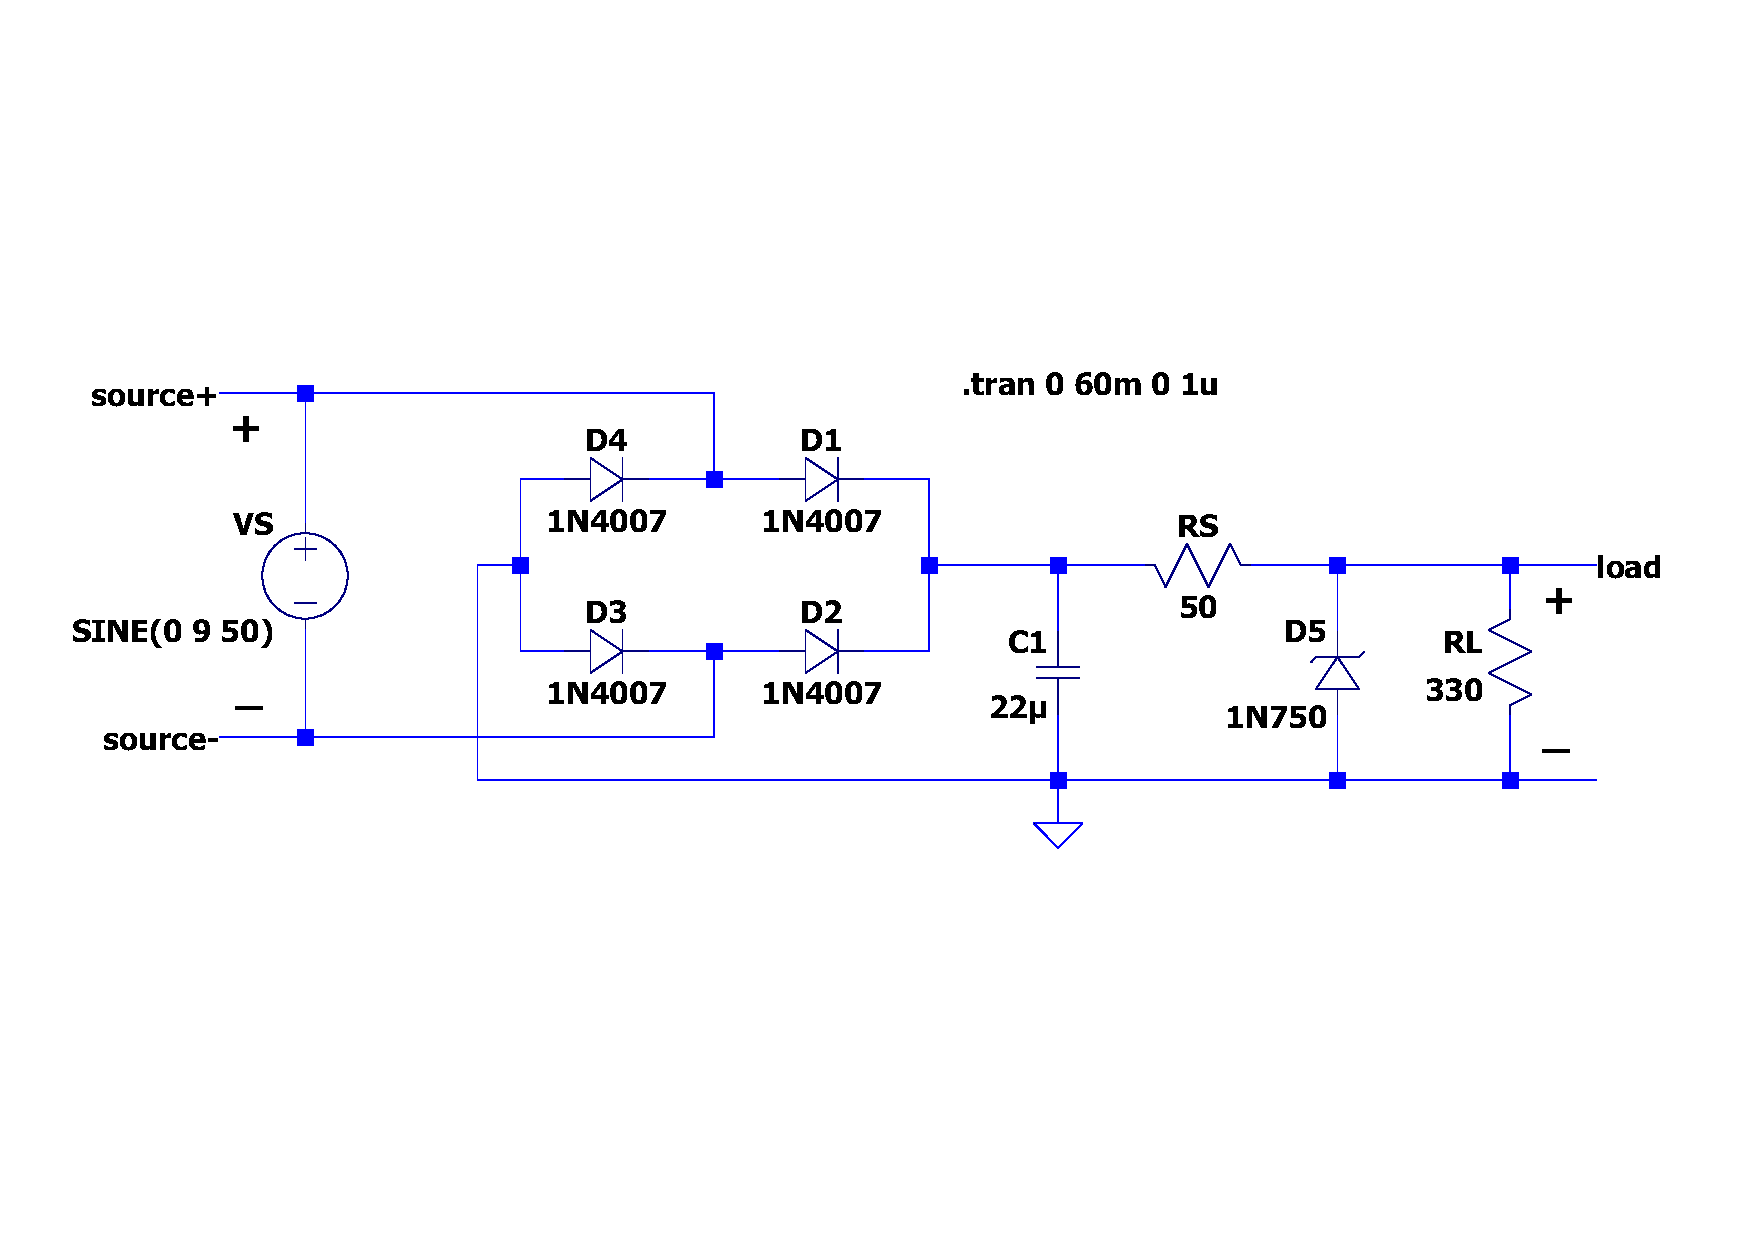
\includegraphics[width=0.8\textwidth]{./figures/circuit-2.pdf}
    \caption{Schematic of Zener diode regulator circuit}
    \label{fig:circuit-2}
\end{figure}

\vspace{0.5cm}

\begin{figure}[H]
    \centering
    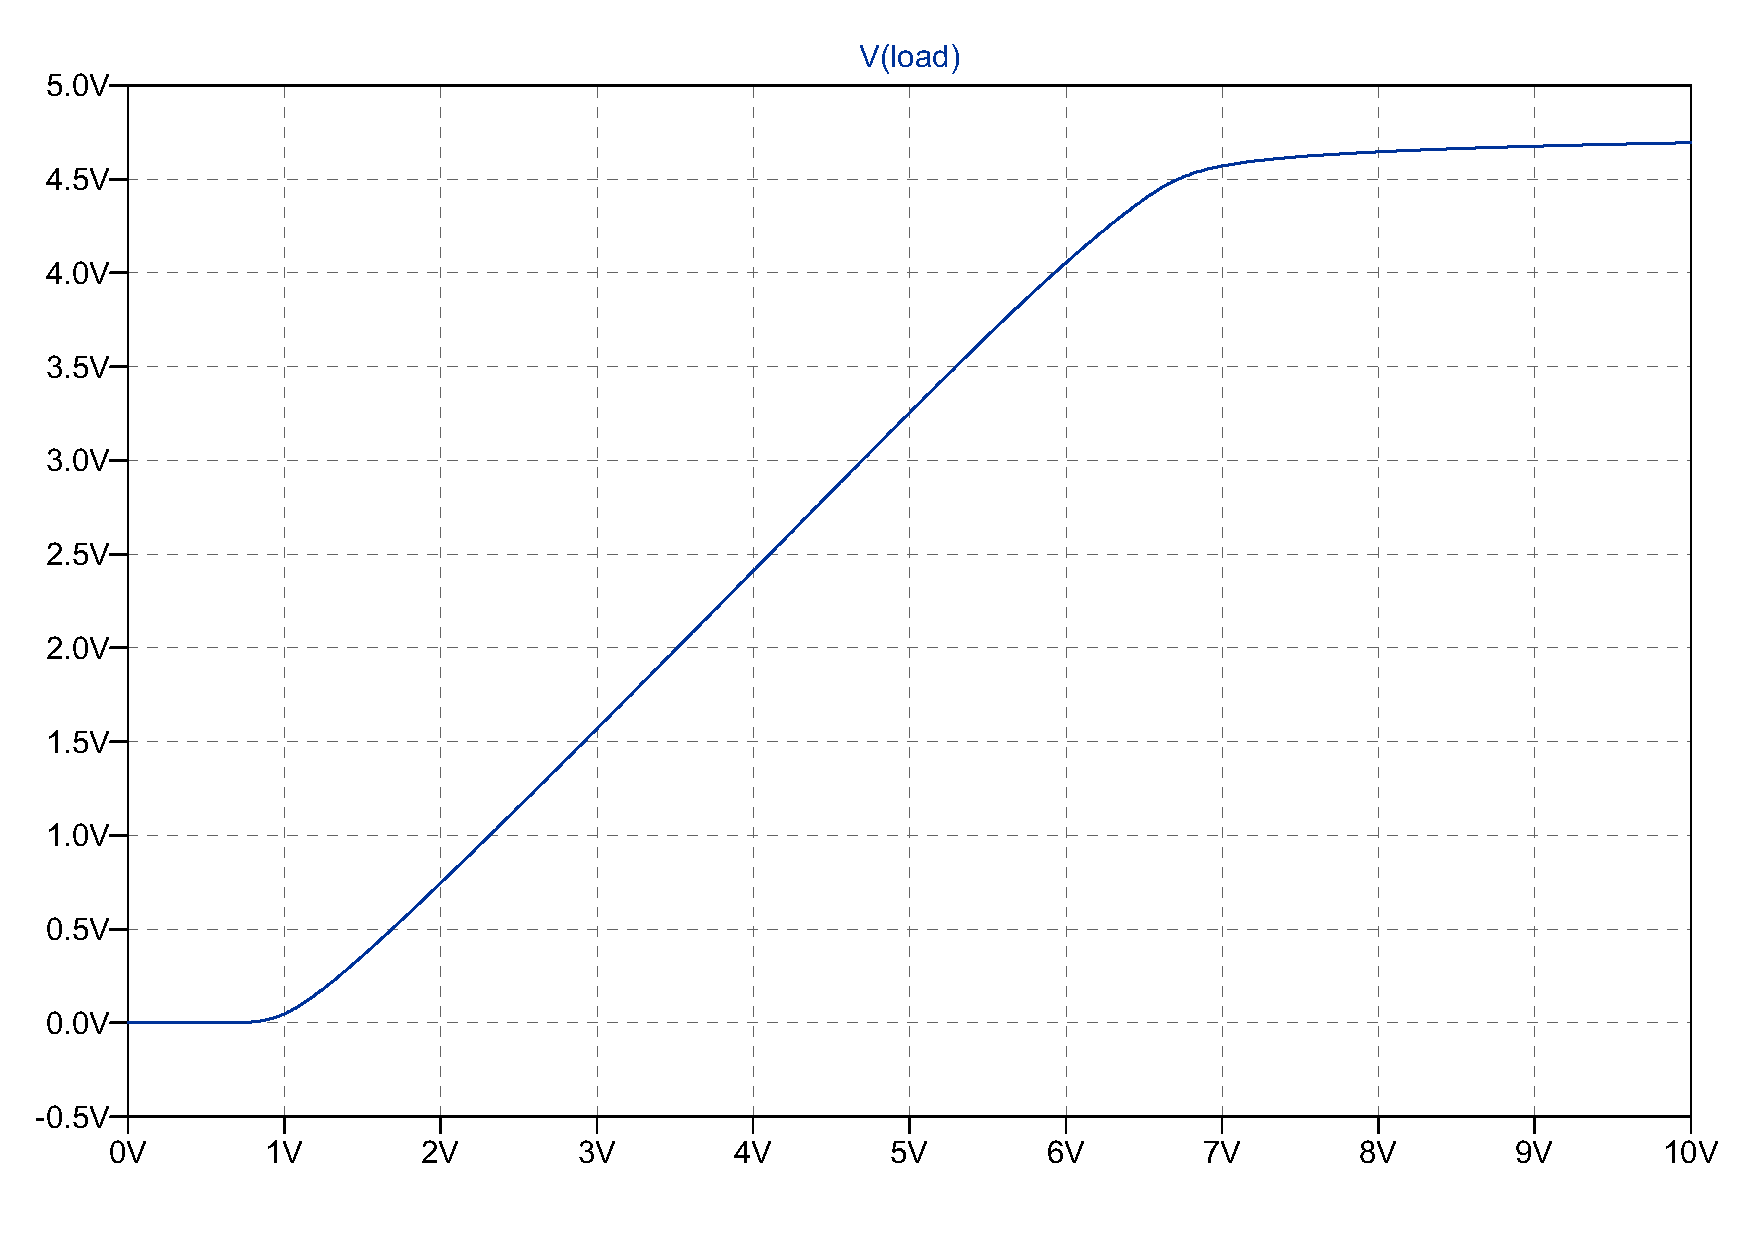
\includegraphics[width=0.8\textwidth]{./figures/plot-2.pdf}
    \caption{Regulated output voltage ($v_L$) as a function of the swept input voltage ($v_S$)}
    \label{fig:plot-2}
\end{figure}

\begin{figure}[H]
    \centering
    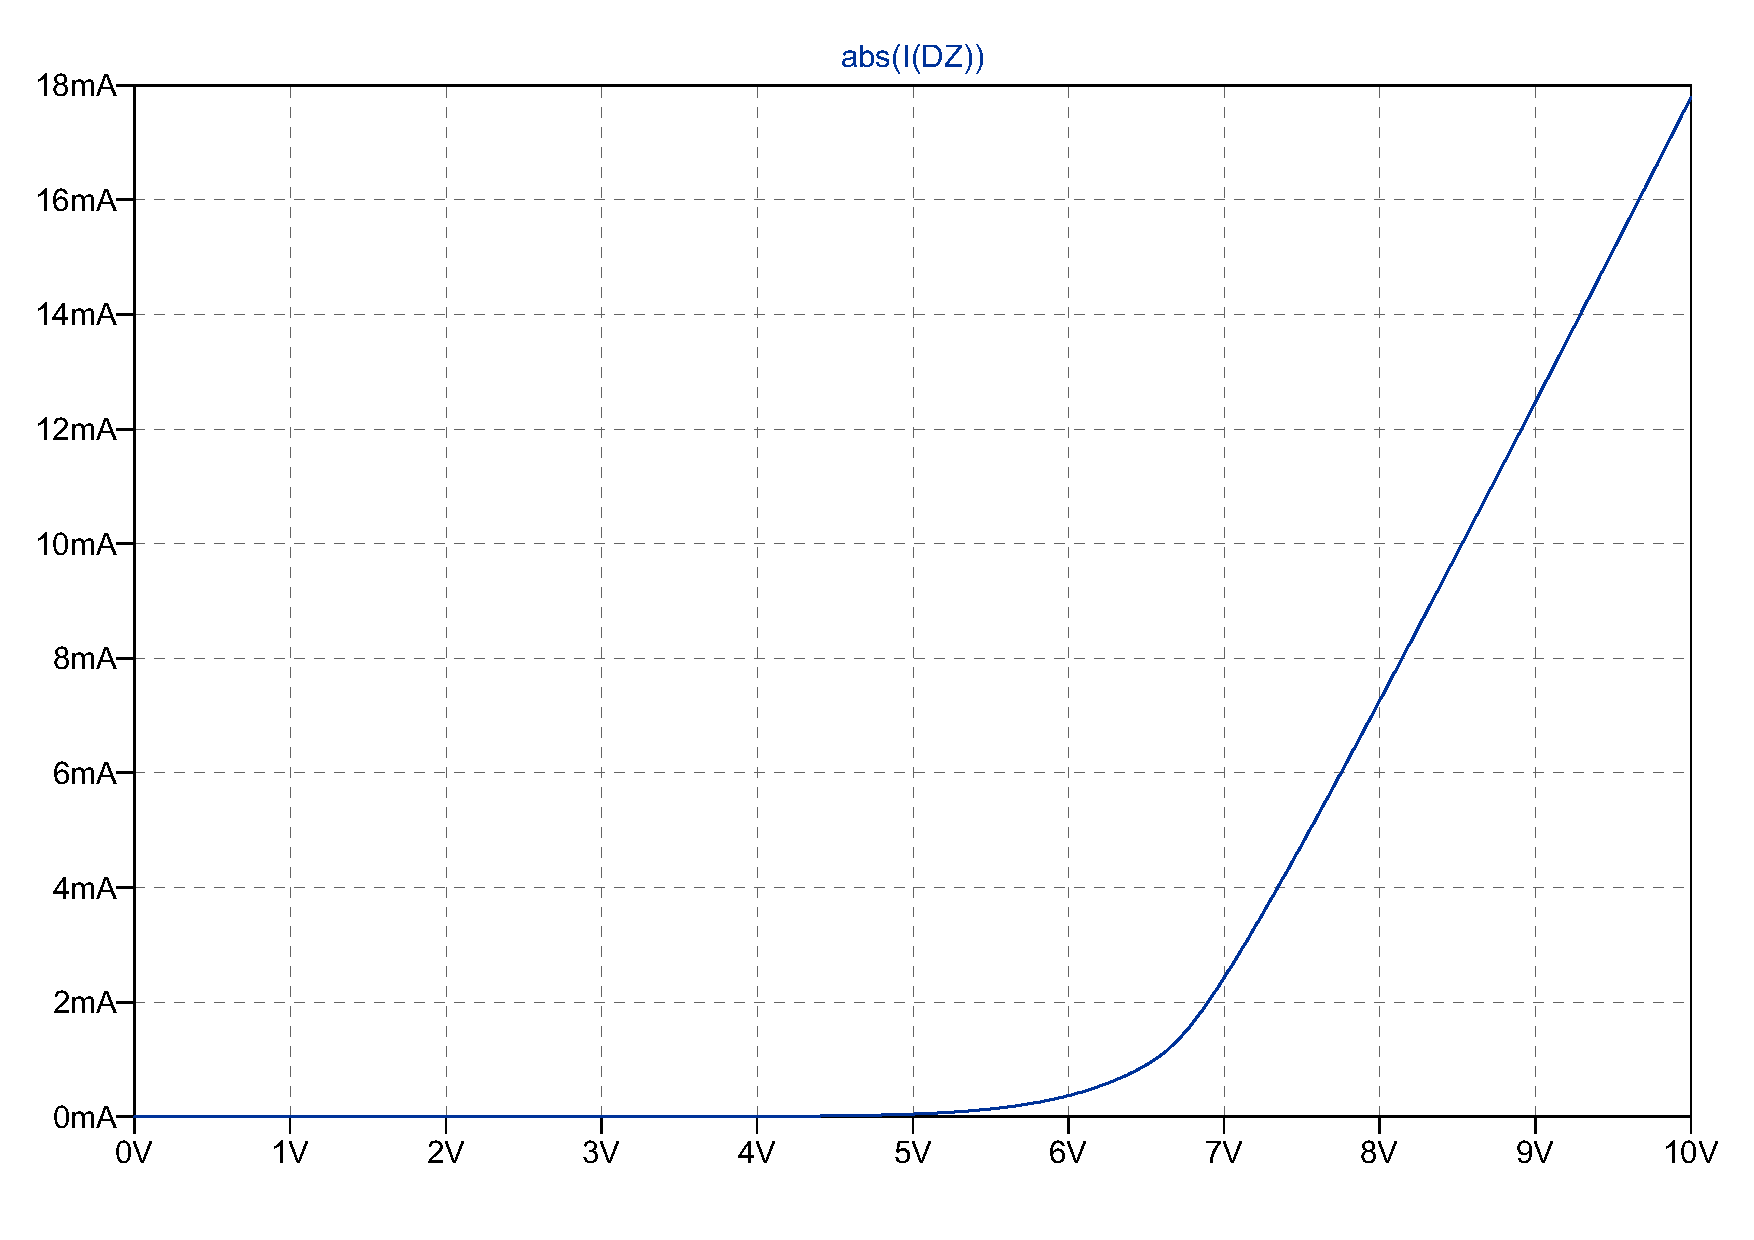
\includegraphics[width=0.8\textwidth]{./figures/plot-3.pdf}
    \caption{Zener breakdown-current magnitude ($i_Z$) versus the swept input voltage ($v_S$)}
    \label{fig:plot-3}
\end{figure}

\subsubsection*{5.3.1 Questions}
\textbf{a.) } \textit{Determine the DC output voltage and the Zener diode current.}\par
\vspace{0.2cm}
\begin{center}
    \begin{tabular}{|c|c|c|}
    \hline
    Breakdown Voltage ($V_Z$) & $V_{o,DC}$ & $I_Z$ \\ \hline
    \VZ & \VoDC & \IZ \\ \hline
    \end{tabular}
\end{center}

\vspace{0.5cm}
\textbf{b.) } \textit{Determine the approximate input voltage at which regulation begins and the regulated output voltage.}\par
-- The regulation starts at breakdown voltage of the Zener diode ($V_Z = \VZ$) as the diode limits the output voltage from exceeding it.

\vspace{0.5cm}
\textbf{c.) } \textit{Include the plots of $v_L$ and the Zener breakdown-current magnitude $i_Z$ versus $v_C$ in your prelab report.}\par
-- The mentioned plots of the example circuit are given in \autoref{fig:plot-2} and \autoref{fig:plot-3}.